\documentclass[12pt,a4paper]{article}
\usepackage[utf8]{inputenc}
\usepackage[catalan]{babel}
\usepackage{graphicx}
\usepackage{geometry}
\usepackage{fancyhdr}
\usepackage{tabularx}
\usepackage{lastpage}
\usepackage{enumitem}
\usepackage{amsmath}
\usepackage{tikz}
\usepackage{hyperref}
\hypersetup{colorlinks=true, urlcolor=blue}

% 1. MARGES I CAPÇALERA ORIGINALS RECUPERATS
\geometry{top=4cm, bottom=3cm, left=2cm, right=2cm, headheight=2.5cm}

\pagestyle{fancy}
\fancyhf{}
% Logos recuperats de la plantilla original
\fancyhead[L]{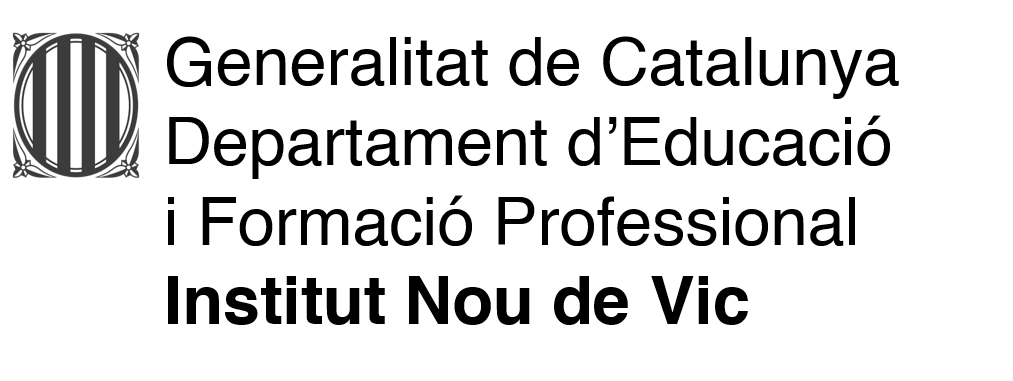
\includegraphics[height=1.8cm]{Logo_Departament.png}} 
\fancyhead[R]{
\includegraphics[height=1.8cm]{Logo_Institut.png}}
\fancyhead[C]{\textbf{Guia de Dibuix Tècnic:\\La Funció Sinus}}

\fancyfoot[L]{}
\fancyfoot[C]{Pàgina \thepage\ de \pageref{LastPage}}
\fancyfoot[R]{}

\renewcommand{\headrulewidth}{0.4pt}

\begin{document}

% --- CAPÇALERA D'IDENTIFICACIÓ ---
\begingroup
\renewcommand{\arraystretch}{2.2}
\begin{tabularx}{\textwidth}{|X|p{4cm}|}
    \hline
    \textbf{Nom i cognoms:} & \textbf{Grup:} \\ \hline
    \textbf{Activitat:} Representació de les funcions $\sin{x}$ i $\cos{x}$  & \textbf{Data:} \\ \hline
\end{tabularx}
\endgroup

\vspace{0.8cm}

\section*{Pas 1: Funció $\sin{x}$ - Preparació del full (en horitzontal)}

Tot i que aquesta guia és vertical, tu has de treballar amb el teu \textbf{full DIN-A4 en posició horitzontal}. Segueix aquestes mides exactes per situar el dibuix d'esquerra a dreta:

\begin{itemize}
    \item \textbf{Centre i Radi:} Situa el centre de la circumferència a \textbf{5 cm del marge esquerre} i centrat verticalment al full. Dibuixa la circumferència amb un \textbf{radi de 4 cm}.
    \item \textbf{Escala horitzontal:} Traça l'eix horitzontal infinit cap a la dreta. L'ona començarà \textbf{0,5 cm a la dreta} de l'extrem del cercle. Des d'aquest punt (el teu nou $0$), mesura \textbf{9 cm per situar $\pi$} i \textbf{18 cm per situar $2\pi$}.
\end{itemize}

\begin{center}
\begin{tikzpicture}[scale=0.45] 
    % El full físic de l'alumne (horitzontal)
    \draw[thick, fill=gray!5] (0,0) rectangle (29.7, 21);
    \node at (14.8, 20) [below] {\textbf{EL TEU FULL (Posició horitzontal)}};
    
    % Indicació de marge
    \draw[<->] (0,15) -- (5,15);
    \node at (2.5, 15.5) {\small 5 cm};
    
    % Dibuix base
    \draw[thick, blue] (5, 10.5) circle (4); % Cercle
    \draw[thick, ->] (1, 10.5) -- (28.5, 10.5) node[right] {Eix $x$};
    
    
    % Nou punt d'origen de la sinusoide (0.5 cm a la dreta del límit del cercle)
    % Límit cercle: 5 + 4 = 9. Nou origen: 9.5
    \fill[black] (9.5, 10.5) circle (3pt) node[above left] {$0$};

    % Escala pi arrencant des de x=9.5
    \draw[|-|] (9.5, 8) -- (18.5, 8);
    \node at (14, 7.5) {\small 9 cm = $\pi$};
    \draw[|-|] (18.5, 8) -- (27.5, 8);
    \node at (23, 7.5) {\small 9 cm més = $2\pi$};
    
    % Radi
    \draw[<->] (5, 10.5) -- (5+4, 10.5);
    \node at (7, 11) [blue] {\small $r=4$ cm};
\end{tikzpicture}
\end{center}

\newpage
\section*{Pas 2: Determinació dels angles a la circumferència}

\subsection*{2.1. Els $90^\circ$ i $270^\circ$ (La Mediatriu)}
Tens un diàmetre horitzontal sencer traçat ($0^\circ$ a la dreta i $180^\circ$ a l'esquerra). Obre el compàs una mica més de la meitat d'aquest diàmetre, punxa a cadascun dels dos extrems i traça dos arcs que es tallin a dalt i a baix. La línia que uneix aquestes creus et donarà l'eix vertical perfecte ($90^\circ$ i $270^\circ$).

\begin{center}
\begin{tikzpicture}[scale=1]
    \draw[thick] (0,0) circle (2);
    \draw[thick, ->] (-3,0) -- (3,0) node[right] {$x$};
    
    % Arcs de la mediatriu (oberts més que el radi)
    \begin{scope}
        \clip (-1.5,-3) rectangle (1.5,3);
        \draw[cyan, dashed, thick] (-2,0) circle (3);
        \draw[cyan, dashed, thick] (2,0) circle (3);
    \end{scope}
    
    % Punts i eix Y
    \fill[black] (0, 2.236) circle (2pt);
    \fill[black] (0, -2.236) circle (2pt);
    \draw[thick, red, ->] (0,-2.8) -- (0,2.8) node[above] {$y$ ($90^\circ$)};
    
    % Llegendes
    \fill[red] (2,0) circle (2pt);
    \node[text=red, scale=0.8] at (2.5, -0.4) {Punxa a $0^\circ$};
    \fill[red] (-2,0) circle (2pt);
    \node[text=red, scale=0.8] at (-2.5, -0.4) {Punxa a $180^\circ$};
\end{tikzpicture}
\end{center}

\subsection*{2.2. Els $45^\circ$ (La Bisectriu)}
Per trobar l'angle de $45^\circ$ ($\pi/4$), traça la bisectriu del primer quadrant. Punxa als $0^\circ$ i fes un arc a l'espai buit del quadrant. Amb la mateixa obertura, punxa als $90^\circ$ i fes un altre arc que el talli. Uneix la creu amb el centre de la circumferència.

\begin{center}
\begin{tikzpicture}[scale=1]
    \draw[thick] (0,0) circle (2);
    \draw[thick, ->] (-2.5,0) -- (2.5,0) node[right] {$x$};
    \draw[thick, ->] (0,-2.5) -- (0,2.5) node[above] {$y$};
    
    % Arcs per la bisectriu
    \begin{scope}
        \clip (0.5,0.5) rectangle (2.5,2.5);
        \draw[cyan, thick, dashed] (2,0) circle (2.2);
        \draw[cyan, thick, dashed] (0,2) circle (2.2);
    \end{scope}
    
    % Bisectriu i punts
    \draw[thick, blue] (0,0) -- (1.8,1.8);
    \fill[black] ({2*cos(45)}, {2*sin(45)}) circle (2pt) node[above right] {$\frac{\pi}{4}$};
    
    \fill[red] (2,0) circle (2pt);
    \node[text=red, scale=0.8] at (2.5, -0.3) {Punxa a $0^\circ$};
    \fill[red] (0,2) circle (2pt);
    \node[text=red, scale=0.8] at (-0.6, 2) {Punxa a $90^\circ$};
\end{tikzpicture}
\end{center}

\textit{Nota: Ara repeteix aquests procediments de bisectriu pel 2n, 3r i 4t quadrant per obtenir les divisions en quarts de $\pi$.}

\newpage
\subsection*{2.3. Els $30^\circ$ i $60^\circ$ (Arc de radi)}
Obre el compàs amb la \textbf{mesura exacta del radi de la circumferència (4 cm)} i no el moguis gens. 
\begin{itemize}[noitemsep]
    \item Punxa als $0^\circ$ i marca la circumferència cap a dalt per trobar els \textbf{60º} ($\pi/3$).
    \item Punxa als $90^\circ$ i marca la circumferència cap a la dreta per trobar els \textbf{30º} ($\pi/6$).
\end{itemize}

\begin{center}
\begin{tikzpicture}[scale=1.2] % He augmentat una miqueta l'escala perquè quedi més clar
    % Eixos
    \draw[thick, ->] (-2.5,0) -- (2.5,0) node[right] {$x$};
    \draw[thick, ->] (0,-2.5) -- (0,2.5) node[above] {$y$};
    
    % Cercle principal
    \draw[thick] (0,0) circle (2);
    
    % --- CONSTRUCCIÓ AMB COMPÀS ---
    % Arc taronja: Centre a (2,0). Comencem a dibuixar des del (0,0) (que equival a l'angle 180)
    \draw[orange, thick, dashed] (0,0) arc (180:110:2); 
    
    % Arc lila: Centre a (0,2). Comencem a dibuixar des del (0,0) (que equival a l'angle -90)
    \draw[purple, thick, dashed] (0,0) arc (-90:-20:2); 
    
    % Línies dels angles
    \draw[thick] (0,0) -- ({2.3*cos(60)}, {2.3*sin(60)});
    \draw[thick] (0,0) -- ({2.3*cos(30)}, {2.3*sin(30)});
    
    % Punts d'intersecció i etiquetes (ajustades perquè no es trepitgin)
    \fill[black] ({2*cos(60)}, {2*sin(60)}) circle (2pt) node[above right] {$\frac{\pi}{3}$};
    \fill[black] ({2*cos(30)}, {2*sin(30)}) circle (2pt) node[right, yshift=2mm] {$\frac{\pi}{6}$};
    
    % Punts on es "punxa" el compàs
    \fill[red] (2,0) circle (2.5pt);
    \fill[red] (0,2) circle (2.5pt);
\end{tikzpicture}
\end{center}

\textit{Nota: Ara repeteix aquest procediment d'arc de radi punxant des dels extrems dels $180^\circ$ i $270^\circ$ per marcar la resta d'angles als altres tres quadrants.}

\subsection*{Resultat Final del Pas 2}
Abans de continuar, comprova que el teu dibuix s'assembli a aquest. Has de tenir tota la circumferència dividida i etiquetada en el teu full horitzontal:

\begin{center}
\begin{tikzpicture}[scale=0.45] 
    % El full físic de l'alumne
    \draw[thick, fill=gray!5] (0,0) rectangle (29.7, 21);
    \node at (14.8, 20) [below] {\textbf{EL TEU FULL (Cercle completat)}};
    
    
    
    % Dibuix base: Circumferència i Eix X
    \draw[thick, blue] (5, 10.5) circle (4); 
    \draw[thick, ->] (1, 10.5) -- (28.5, 10.5) node[right] {Eix $x$};
    
    % Punt central de referència (opcional, una petita creu)
    \draw[gray] (4.8, 10.5) -- (5.2, 10.5);
    \draw[gray] (5, 10.3) -- (5, 10.7);

    % Marques dels angles (talls de compàs) i etiquetes en radiants
    \foreach \a/\t in {
        30/\frac{\pi}{6}, 45/\frac{\pi}{4}, 60/\frac{\pi}{3}, 90/\frac{\pi}{2},
        120/\frac{2\pi}{3}, 135/\frac{3\pi}{4}, 150/\frac{5\pi}{6}, 180/\pi,
        210/\frac{7\pi}{6}, 225/\frac{5\pi}{4}, 240/\frac{4\pi}{3}, 270/\frac{3\pi}{2},
        300/\frac{5\pi}{3}, 315/\frac{7\pi}{4}, 330/\frac{11\pi}{6}
    } {
        % Dibuixa un petit arc (marca) que creua el perímetre
        \draw[thick, black] ({5+3.8*cos(\a)}, {10.5+3.8*sin(\a)}) -- ({5+4.2*cos(\a)}, {10.5+4.2*sin(\a)});
        
        % Etiqueta en radiants
        \node[scale=0.85, text=black] at ({5+5.1*cos(\a)}, {10.5+5.1*sin(\a)}) {$\t$};
    }
    
    % Marca específica per al 0/2pi (perquè no quedi buit a la dreta)
    \draw[thick, black] (8.8, 10.5) -- (9.2, 10.5);
    \node[scale=0.85, text=black] at (10, 10.5) {$0, 2\pi$};

\end{tikzpicture}
\end{center}

\newpage
\section*{Pas 3: Projecció de la Sinusoide (Pas per pas)}

Ara donarem sentit a cadascuna de les marques traslladant-les de la circumferència cap a la gràfica estesa. Aquesta taula ens recorda el valor exacte de la funció sinus per a cada angle clau. Recorda que el valor del sinus correspon a l'altura (coordenada $y$) respecte al radi:

\vspace{0.3cm}
\begin{center}
\renewcommand{\arraystretch}{2}
\begin{tabular}{|c|c|c|}
\hline
\textbf{Angle (graus)} & \textbf{Angle (radiants)} & \textbf{Valor exacte $f(x) = \sin(x)$} \\ \hline
$0^\circ$ & $0$ & $0$ \\ \hline
$30^\circ$ & $\frac{\pi}{6}$ & $\frac{1}{2}$ \\ \hline
$45^\circ$ & $\frac{\pi}{4}$ & $\frac{\sqrt{2}}{2}$ \\ \hline
$60^\circ$ & $\frac{\pi}{3}$ & $\frac{\sqrt{3}}{2}$ \\ \hline
$90^\circ$ & $\frac{\pi}{2}$ & $1$ (Radi màxim) \\ \hline
$120^\circ$ & $\frac{2\pi}{3}$ & $\frac{\sqrt{3}}{2}$ \\ \hline
$135^\circ$ & $\frac{3\pi}{4}$ & $\frac{\sqrt{2}}{2}$ \\ \hline
$\dots$ & $\dots$ & $\dots$ \\ \hline
$330^\circ$ & $\frac{11\pi}{6}$ & $-\frac{1}{2}$ \\ \hline
\end{tabular}
\end{center}
\vspace{0.3cm}

Com no podem mesurar fàcilment amb el regle valors irracionals com $\frac{\sqrt{2}}{2}$, el que farem serà traslladar geomètricament aquesta funció a l'eix horitzontal estès.

\subsection*{3.1. Dibuixar l'eix vertical i dividir l'eix horitzontal}
Agafa el teu regle físic i ves al full on has dibuixat la circumferència. Fes una petita marca a l'eix horitzontal situada a \textbf{exactament 0,5 cm a la dreta} de l'extrem de la circumferència (la marca dels $0^\circ$).

En aquest nou punt:
\begin{itemize}[noitemsep]
    \item Fes servir l'escaire recolzat al cartabó per traçar una línia perfectament perpendicular. Aquest serà \textbf{l'eix vertical} (eix $y$) de la teva sinusoide.
    \item Posa el zero del teu regle en aquesta nova intersecció. Com que hem establert que $\pi = 9\text{ cm}$, el teu eix horitzontal mesurarà \textbf{18 cm} fins a $2\pi$. Fes servir fraccions de 9 cm per situar cadascun dels angles al llarg de la línia:
\end{itemize}

\begin{itemize}[noitemsep]
    \item $\pi/6$ estarà a \textbf{1,5 cm}.
    \item $\pi/4$ estarà a \textbf{2,25 cm} (entre el mil·límetre 2 i 3).
    \item $\pi/3$ estarà a \textbf{3 cm}.
    \item $\pi/2$ estarà a \textbf{4,5 cm}.
\end{itemize}

\vspace{0.2cm}
Hauria de quedar una cosa així al teu full, preparat per començar a dibuixar la corba:

\begin{center}
\begin{tikzpicture}[scale=0.45] 
    % 1. REPRESENTACIÓ DEL FULL (DIN-A4 Horitzontal)
    \draw[thick, fill=gray!5] (0,0) rectangle (29.7, 21);
    \node at (14.8, 20) [below] {\textbf{ESTAT DEL FULL AL FINAL DEL PAS 3.1}};
        
    % 2. LA CIRCUMFERÈNCIA
    \draw[thick, blue] (5, 10.5) circle (4); 
    
    % Marques dels angles a la circumferència
    \foreach \a/\t in {
        30/\frac{\pi}{6}, 45/\frac{\pi}{4}, 60/\frac{\pi}{3}, 90/\frac{\pi}{2},
        120/\frac{2\pi}{3}, 135/\frac{3\pi}{4}, 150/\frac{5\pi}{6}, 180/\pi,
        210/\frac{7\pi}{6}, 225/\frac{5\pi}{4}, 240/\frac{4\pi}{3}, 270/\frac{3\pi}{2},
        300/\frac{5\pi}{3}, 315/\frac{7\pi}{4}, 330/\frac{11\pi}{6}
    } {
        \draw[thick, black] ({5+3.8*cos(\a)}, {10.5+3.8*sin(\a)}) -- ({5+4.2*cos(\a)}, {10.5+4.2*sin(\a)});
        \node[scale=0.7, text=black] at ({5+5*cos(\a)}, {10.5+5*sin(\a)}) {$\t$};
    }

    % 3. EIXOS DE LA FUNCIÓ (Pas 3.1)
    % L'eix X global
    \draw[->, ultra thick] (5, 10.5) -- (28.5, 10.5) node[right] {Eix $x$};
    
    % Nou eix vertical a x=9.5 (0.5cm de l'extrem del cercle que és a 9)
    \draw[thick, red, ->] (9.5, 6) -- (9.5, 15) node[above] {Eix $y$};
    \fill[black] (9.5, 10.5) circle (2.5pt) node[below left] {$0$};
    
    % Divisions basades en pi = 9cm arrencant de x=9.5
    \foreach \dist/\t in {
        1.5/\frac{\pi}{6}, 2.25/\frac{\pi}{4}, 3/\frac{\pi}{3}, 4.5/\frac{\pi}{2}, 
        6/\frac{2\pi}{3}, 6.75/\frac{3\pi}{4}, 7.5/\frac{5\pi}{6}, 9/\pi,
        10.5/\frac{7\pi}{6}, 11.25/\frac{5\pi}{4}, 12/\frac{4\pi}{3}, 13.5/\frac{3\pi}{2},
        15/\frac{5\pi}{3}, 15.75/\frac{7\pi}{4}, 16.5/\frac{11\pi}{6}, 18/2\pi
    } {
        \draw[thick, blue] ({9.5+\dist}, 10.7) -- ({9.5+\dist}, 10.3) node[below=8pt, text=black, scale=0.75] {$\t$};
    }

\end{tikzpicture}
\end{center}
\newpage
\subsection*{3.2. Traslladar el primer punt ($\pi/6$)}

Ara trobarem l'alçada exacta del primer punt de la gràfica. Per fer-ho, treballarem amb l'escaire i el cartabó per assegurar línies perfectament rectes:

\begin{enumerate}
    \item \textbf{La línia horitzontal (Paral·lela):} Busca la marca de $\pi/6$ ($30^\circ$) al perímetre de la teva circumferència. Fent servir l'escaire recolzat sobre el cartabó per fer paral·leles a l'eix horitzontal, traça una línia discontínua llarga cap a la dreta.
    
    \item \textbf{La línia vertical (Perpendicular):} Ara ves a la marca de $\pi/6$ que has situat a l'eix de la teva sinusoide (a 1,5 cm de l'eix vertical). Utilitza l'escaire per pujar una línia discontínua perpendicular.
    
    \item \textbf{El punt d'intersecció:} El lloc exacte on es creuen aquestes dues línies és el teu \textbf{primer punt} de la corba. Marca'l amb un punt clar.
\end{enumerate}

\begin{center}
\begin{tikzpicture}[scale=0.5] 
    % REPRESENTACIÓ DEL FULL
    \draw[thick, fill=gray!5] (0,0) rectangle (29.7, 18);
    
    % CIRCUMFERÈNCIA (Simplificada amb només pi/6 i 5pi/6)
    \draw[thick, blue] (5, 9) circle (4); 
    \draw[thick, ->] (1, 9) -- (28.5, 9) node[right] {Eix $x$};
    
    % Marques d'angles rellevants
    \foreach \a/\t in {30/\frac{\pi}{6}, 150/\frac{5\pi}{6}} {
        \draw[thick, black] ({5+3.8*cos(\a)}, {9+3.8*sin(\a)}) -- ({5+4.2*cos(\a)}, {9+4.2*sin(\a)});
        \node[scale=0.8, text=black] at ({5+5*cos(\a)}, {9+5*sin(\a)}) {$\t$};
    }

    % EIXOS DE LA SINUSOIDE
    % Eix Y situat a 0.5cm de la vora del cercle (9.5)
    \draw[thick, red, ->] (9.5, 4.5) -- (9.5, 13.5) node[above] {Eix $y$};
    \fill[black] (9.5, 9) circle (2.5pt) node[below left] {$0$};
    
    % MARQUES EIX X (Simplificades)
    % pi/6 a 1.5cm de l'origen (9.5 + 1.5 = 11)
    % 5pi/6 a 7.5cm de l'origen (9.5 + 7.5 = 17)
    \draw[thick, blue] (11, 9.2) -- (11, 8.8) node[below=8pt, text=black, scale=0.8] {$\frac{\pi}{6}$};
    \draw[thick, blue] (17, 9.2) -- (17, 8.8) node[below=8pt, text=black, scale=0.8] {$\frac{5\pi}{6}$};
    \draw[thick, blue] (18.5, 9.2) -- (18.5, 8.8) node[below=8pt, text=black, scale=0.8] {$\pi$};

    % TRACATS GEOMÈTRICS (Línies discontínues)
    % Paral·lela horitzontal llarga des de pi/6 (altura = 9 + 4*sin(30) = 11)
    \draw[dashed, cyan, thick] ({5+4*cos(30)}, 11) -- (22, 11);
    
    % Perpendicular des de pi/6 a l'eix X (x = 11)
    \draw[dashed, orange, thick] (11, 9) -- (11, 11);
    
    % Punt d'intersecció
    \fill[red] (11, 11) circle (3.5pt) node[above right, text=black, scale=0.8] {\textbf{Punt 1}};

\end{tikzpicture}
\end{center}

\textit{\textbf{Truc:} Si t'hi fixes, la línia horitzontal que has traçat passa exactament a la mateixa altura que el punt $\frac{5\pi}{6}$ de la circumferència. Això vol dir que, més endavant, quan hagis de situar el punt de $\frac{5\pi}{6}$ a la gràfica, ja tindràs l'altura marcada!}

\newpage

\subsection*{3.3. Traslladar els punts de $\pi/4$ i $3\pi/4$}

Ara que ja has vist com funciona, repeteix el mateix procés per a la marca de $\pi/4$ ($45^\circ$). Fixa't que pots allargar la línia horitzontal cap a l'esquerra fins al $3\pi/4$ ($135^\circ$) i cap a la dreta fins a la teva gràfica, ja que comparteixen exactament la mateixa alçada.

Traça la paral·lela des d'aquests angles a la circumferència i puja les perpendiculars des de les teves marques de l'eix horitzontal (a 2,25 cm i 6,75 cm de l'eix vertical).

\begin{center}
\begin{tikzpicture}[scale=0.5] 
    % REPRESENTACIÓ DEL FULL
    \draw[thick, fill=gray!5] (0,0) rectangle (29.7, 18);
    
    % CIRCUMFERÈNCIA
    \draw[thick, blue] (5, 9) circle (4); 
    \draw[thick, ->] (1, 9) -- (28.5, 9) node[right] {Eix $x$};
    
    % Marques d'angles rellevants (els anteriors i els nous)
    \foreach \a/\t in {30/\frac{\pi}{6}, 45/\frac{\pi}{4}, 135/\frac{3\pi}{4}, 150/\frac{5\pi}{6}} {
        \draw[thick, black] ({5+3.8*cos(\a)}, {9+3.8*sin(\a)}) -- ({5+4.2*cos(\a)}, {9+4.2*sin(\a)});
        \node[scale=0.8, text=black] at ({5+5.1*cos(\a)}, {9+5.1*sin(\a)}) {$\t$};
    }

    % EIXOS DE LA SINUSOIDE
    \draw[thick, red, ->] (9.5, 4.5) -- (9.5, 13.5) node[above] {Eix $y$};
    \fill[black] (9.5, 9) circle (2.5pt) node[below left] {$0$};
    
    % MARQUES EIX X
    % pi/6 (11), pi/4 (11.75), 3pi/4 (16.25), 5pi/6 (17)
    \draw[thick, blue] (11, 9.2) -- (11, 8.8) node[below=8pt, text=black, scale=0.7] {$\frac{\pi}{6}$};
    \draw[thick, blue] (11.75, 9.2) -- (11.75, 8.8) node[below=8pt, text=black, scale=0.7] {$\frac{\pi}{4}$};
    \draw[thick, blue] (16.25, 9.2) -- (16.25, 8.8) node[below=8pt, text=black, scale=0.7] {$\frac{3\pi}{4}$};
    \draw[thick, blue] (17, 9.2) -- (17, 8.8) node[below=8pt, text=black, scale=0.7] {$\frac{5\pi}{6}$};
    \draw[thick, blue] (18.5, 9.2) -- (18.5, 8.8) node[below=8pt, text=black, scale=0.7] {$\pi$};

    % PUNTS ANTERIORS (Ja consolidats)
    \fill[gray] (11, {9+4*sin(30)}) circle (3pt);
    \fill[gray] (17, {9+4*sin(150)}) circle (3pt);

    % NOUS TRACATS GEOMÈTRICS (Línies discontínues per 45 i 135)
    % Paral·lela horitzontal llarga des de 135 passant per 45 cap a la gràfica
    \draw[dashed, cyan, thick] ({5+4*cos(135)}, {9+4*sin(45)}) -- (18, {9+4*sin(45)});
    
    % Perpendiculars a l'eix X
    \draw[dashed, orange, thick] (11.75, 9) -- (11.75, {9+4*sin(45)});
    \draw[dashed, orange, thick] (16.25, 9) -- (16.25, {9+4*sin(135)});
    
    % Nous punts d'intersecció
    \fill[red] (11.75, {9+4*sin(45)}) circle (3.5pt);
    \fill[red] (16.25, {9+4*sin(135)}) circle (3.5pt);

\end{tikzpicture}
\end{center}

\newpage
\subsection*{3.4. Traslladar els punts de $\pi/3$ i $2\pi/3$}

Finalitzem el primer bloc de punts amb l'angle de $60^\circ$ ($\pi/3$) i el seu simètric de $120^\circ$ ($2\pi/3$). 

Repeteix el procediment: traça la paral·lela horitzontal que uneixi els dos angles de la circumferència i projecta-la cap a la dreta. Després, puja les perpendiculars des de les marques de l'eix horitzontal situades a \textbf{3 cm} i \textbf{6 cm} de l'eix vertical.

\begin{center}
\begin{tikzpicture}[scale=0.5] 
    % REPRESENTACIÓ DEL FULL
    \draw[thick, fill=gray!5] (0,0) rectangle (29.7, 18);
    
    % CIRCUMFERÈNCIA
    \draw[thick, blue] (5, 9) circle (4); 
    \draw[thick, ->] (1, 9) -- (28.5, 9) node[right] {Eix $x$};
    
    % Marques d'angles rellevants (Tots els del 1r i 2n quadrant per coherència)
    \foreach \a/\t in {30/\frac{\pi}{6}, 45/\frac{\pi}{4}, 60/\frac{\pi}{3}, 120/\frac{2\pi}{3}, 135/\frac{3\pi}{4}, 150/\frac{5\pi}{6}} {
        \draw[thick, black] ({5+3.8*cos(\a)}, {9+3.8*sin(\a)}) -- ({5+4.2*cos(\a)}, {9+4.2*sin(\a)});
        \node[scale=0.75, text=black] at ({5+5.1*cos(\a)}, {9+5.1*sin(\a)}) {$\t$};
    }

    % EIXOS DE LA SINUSOIDE
    \draw[thick, red, ->] (9.5, 4.5) -- (9.5, 13.5) node[above] {Eix $y$};
    \fill[black] (9.5, 9) circle (2.5pt) node[below left] {$0$};
    
    % MARQUES EIX X
    % pi/6 (11), pi/4 (11.75), pi/3 (12.5), 2pi/3 (15.5), 3pi/4 (16.25), 5pi/6 (17)
    \foreach \pos/\t in {11/\frac{\pi}{6}, 11.75/\frac{\pi}{4}, 12.5/\frac{\pi}{3}, 15.5/\frac{2\pi}{3}, 16.25/\frac{3\pi}{4}, 17/\frac{5\pi}{6}, 18.5/\pi} {
        \draw[thick, blue] (\pos, 9.2) -- (\pos, 8.8) node[below=8pt, text=black, scale=0.65] {$\t$};
    }

    % PUNTS ANTERIORS (En gris per no distreure)
    \fill[gray!60] (11, {9+4*sin(30)}) circle (3pt);
    \fill[gray!60] (17, {9+4*sin(150)}) circle (3pt);
    \fill[gray!60] (11.75, {9+4*sin(45)}) circle (3pt);
    \fill[gray!60] (16.25, {9+4*sin(135)}) circle (3pt);

    % NOUS TRACATS GEOMÈTRICS (60 i 120)
    % Paral·lela horitzontal llarga
    \draw[dashed, cyan, thick] ({5+4*cos(120)}, {9+4*sin(60)}) -- (17.5, {9+4*sin(60)});
    
    % Perpendiculars a l'eix X
    \draw[dashed, orange, thick] (12.5, 9) -- (12.5, {9+4*sin(60)});
    \draw[dashed, orange, thick] (15.5, 9) -- (15.5, {9+4*sin(120)});
    
    % Nous punts d'intersecció
    \fill[red] (12.5, {9+4*sin(60)}) circle (3.5pt);
    \fill[red] (15.5, {9+4*sin(120)}) circle (3.5pt);

\end{tikzpicture}
\end{center}

\textit{Ja tens gairebé tota la part positiva de l'ona! No oblidis marcar el punt de $\pi/2$ ($90^\circ$), que és el més alt (el radi sencer), i el punt $\pi$ on la corba torna a tocar l'eix horitzontal.}
\textbf{Fes la resta de la corba}

\newpage
\subsection*{3.5. Traçat de la corba (La Sinusoide)}

Un cop hagis traslladat tots els punts de la circumferència a la gràfica (els 12 punts de les divisions més els punts de tall amb l'eix), tindràs l'esquelet complet de la funció sinus.

\begin{itemize}
    \item \textbf{Verificació:} Comprova que els punts dels quadrants 3 i 4 ($210^\circ$ a $330^\circ$) han quedat per sota de l'eix horitzontal, ja que en aquesta zona el sinus és negatiu.
    \item \textbf{El traçat:} Ara, \textbf{a mà alçada}, uneix tots els punts amb una línia suau i contínua. Evita fer angles punxeguts; la sinusoide és una ona arrodonida i fluida.
\end{itemize}

\begin{center}
\begin{tikzpicture}[scale=0.5] 
    % 1. REPRESENTACIÓ DEL FULL
    \draw[thick, fill=gray!5] (0,0) rectangle (29.7, 18);
    
    % 2. CIRCUMFERÈNCIA (Amb totes les marques d'angles com al 3.1)
    \draw[thick, blue] (5, 9) circle (4); 
    \draw[thick, ->] (1, 9) -- (28.5, 9) node[right] {Eix $x$};
    
    \foreach \a/\t in {
        30/\frac{\pi}{6}, 45/\frac{\pi}{4}, 60/\frac{\pi}{3}, 90/\frac{\pi}{2},
        120/\frac{2\pi}{3}, 135/\frac{3\pi}{4}, 150/\frac{5\pi}{6}, 180/\pi,
        210/\frac{7\pi}{6}, 225/\frac{5\pi}{4}, 240/\frac{4\pi}{3}, 270/\frac{3\pi}{2},
        300/\frac{5\pi}{3}, 315/\frac{7\pi}{4}, 330/\frac{11\pi}{6}
    } {
        \draw[thick, black] ({5+3.8*cos(\a)}, {9+3.8*sin(\a)}) -- ({5+4.2*cos(\a)}, {9+4.2*sin(\a)});
        \node[scale=0.65, text=black] at ({5+5*cos(\a)}, {9+5*sin(\a)}) {$\t$};
    }

    % 3. EIXOS DE LA SINUSOIDE
    \draw[thick, red, ->] (9.5, 4.5) -- (9.5, 13.5) node[above] {Eix $y$};
    \fill[black] (9.5, 9) circle (2.5pt) node[below left] {$0$};
    
    % 4. MARQUES I TICKS DE L'EIX HORITZONTAL (Com al 3.1)
    \foreach \dist/\t in {
        1.5/\frac{\pi}{6}, 2.25/\frac{\pi}{4}, 3/\frac{\pi}{3}, 4.5/\frac{\pi}{2}, 
        6/\frac{2\pi}{3}, 6.75/\frac{3\pi}{4}, 7.5/\frac{5\pi}{6}, 9/\pi,
        10.5/\frac{7\pi}{6}, 11.25/\frac{5\pi}{4}, 12/\frac{4\pi}{3}, 13.5/\frac{3\pi}{2},
        15/\frac{5\pi}{3}, 15.75/\frac{7\pi}{4}, 16.5/\frac{11\pi}{6}, 18/2\pi
    } {
        \draw[thick, blue] ({9.5+\dist}, 9.2) -- ({9.5+\dist}, 8.8) node[below=8pt, text=black, scale=0.65] {$\t$};
    }

    % 5. TOTS ELS PUNTS RESULTANTS
    \foreach \a in {0, 30, 45, 60, 90, 120, 135, 150, 180, 210, 225, 240, 270, 300, 315, 330, 360} {
        \pgfmathsetmacro{\posX}{9.5 + (\a * 9 / 180)}
        \pgfmathsetmacro{\posY}{9 + (4 * sin(\a))}
        \fill[red] (\posX, \posY) circle (3.5pt);
    }

\end{tikzpicture}
\end{center}

\textit{\textbf{Consell:} Intenta que el traç sigui d'un sol gest, sense dubtar. Pots fer primer un traç molt fi amb llapis i, quan t'agradi la forma, repassar-lo un retolador fi.}


\newpage
\newpage
\section*{Pas 4: La Funció Cosinus (Repte Independent)}

Ara que ja domines el traçat del sinus, el teu objectiu és representar la funció \textbf{$f(x) = \cos(x)$}. Tot i que la corba té una forma similar, el cosinus mesura la projecció horitzontal de l'angle.

Per poder seguir treballant amb l'escaire i el cartabó fent línies horitzontals, farem un "truc" geomètric: **girarem la circumferència $90^\circ$ cap a l'esquerra.**

\subsection*{4.1. El concepte: Girar la referència}

En girar el cercle, l'eix que abans era horitzontal ara és vertical. Això ens permet que el valor del cosinus es converteixi en una "alçada" que podem projectar fàcilment cap a la dreta.

\begin{center}
\begin{tikzpicture}[scale=0.8]
    % Cercle Sinus
    \begin{scope}[xshift=0cm]
        \draw[thick] (0,0) circle (1.5);
        \draw[->] (-1.8,0) -- (1.8,0);
        \draw[->, red, ultra thick] (0,0) -- (0,1.5) node[midway, left] {$\sin$};
        \node at (0,-2) {\small \textbf{Sinus:} El $0$ és a la dreta};
    \end{scope}

    % Fletxa de gir
    \draw[->, bend left, thick] (2.5,0.5) to node[above] {Gir $90^\circ$} (4.5,0.5);

    % Cercle Cosinus girat
    \begin{scope}[xshift=7cm]
        \draw[thick] (0,0) circle (1.5);
        \draw[->] (0,-1.8) -- (0,1.8);
        \draw[->, blue, ultra thick] (0,0) -- (0,1.5) node[midway, right] {$\cos$};
        \node at (0,-2) {\small \textbf{Cosinus:} El $0$ ara és a dalt};
        \fill[red] (0,1.5) circle (2pt) node[above] {$0$ rad};
    \end{scope}
\end{tikzpicture}
\end{center}

\subsection*{4.2. Guies per a la realització}

\begin{enumerate}
    \item \textbf{Nou origen:} Marca el punt de \textbf{$0$ rad a la part superior} de la circumferència. 
    \item \textbf{Determinació dels angles:} De la mateixa manera que has fet al Pas 2, determina tots els angles clau ($\pi/6, \pi/4, \pi/3 \dots$) a partir del nou origen superior i en sentit antihorari. Hauràs de repetir els mètodes de la mediatriu, la bisectriu i l'arc de radi.
    \item \textbf{Eix horitzontal:} Prepara el teu eix a la part dreta del full mantenint la mateixa escala ($\pi = 9\text{ cm}$).
    \item \textbf{Trasllat de punts:} Ara et toca a tu. Trasllada els punts geomètricament a la gràfica aplicant el que has après. Pensa bé des d'on surt cada línia horitzontal i on ha de creuar-se amb la vertical. Recorda que el cosinus de $0$ no és $0$.
\end{enumerate}

\newpage
\subsection*{4.3. Esquema de preparació del full}

Així ha de quedar el teu full abans de començar a traçar les línies de projecció. Fixa't bé en la posició dels angles a la circumferència girada:

\begin{center}
\begin{tikzpicture}[scale=0.5] 
    % REPRESENTACIÓ DEL FULL
    \draw[thick, fill=gray!5] (0,0) rectangle (29.7, 18);
    
    % CIRCUMFERÈNCIA GIRADA (0 rad a dalt)
    \draw[thick, blue] (5, 9) circle (4); 
    \draw[thick, ->] (1, 9) -- (28.5, 9) node[right] {Eix $x$};
    
    % Angles girats (marques i labels)
    \foreach \a/\t in {
        0/0, 30/\frac{\pi}{6}, 45/\frac{\pi}{4}, 60/\frac{\pi}{3}, 90/\frac{\pi}{2},
        120/\frac{2\pi}{3}, 135/\frac{3\pi}{4}, 150/\frac{5\pi}{6}, 180/\pi,
        210/\frac{7\pi}{6}, 225/\frac{5\pi}{4}, 240/\frac{4\pi}{3}, 270/\frac{3\pi}{2},
        300/\frac{5\pi}{3}, 315/\frac{7\pi}{4}, 330/\frac{11\pi}{6}
    } {
        \draw[thick, black] ({5+3.8*cos(\a+90)}, {9+3.8*sin(\a+90)}) -- ({5+4.2*cos(\a+90)}, {9+4.2*sin(\a+90)});
        \node[scale=0.6, text=black] at ({5+5.1*cos(\a+90)}, {9+5.1*sin(\a+90)}) {$\t$};
    }

    % EIXOS DE LA FUNCIÓ (Buits de punts)
    \draw[thick, red, ->] (9.5, 4.5) -- (9.5, 14.5) node[above] {Eix $y$};
    \fill[black] (9.5, 9) circle (2.5pt) node[below left] {$0$};
    
    % MARQUES EIX X (Ticks complets)
    \foreach \dist/\t in {
        1.5/\frac{\pi}{6}, 2.25/\frac{\pi}{4}, 3/\frac{\pi}{3}, 4.5/\frac{\pi}{2}, 
        6/\frac{2\pi}{3}, 6.75/\frac{3\pi}{4}, 7.5/\frac{5\pi}{6}, 9/\pi,
        10.5/\frac{7\pi}{6}, 11.25/\frac{5\pi}{4}, 12/\frac{4\pi}{3}, 13.5/\frac{3\pi}{2},
        15/\frac{5\pi}{3}, 15.75/\frac{7\pi}{4}, 16.5/\frac{11\pi}{6}, 18/2\pi
    } {
        \draw[thick, blue] ({9.5+\dist}, 9.2) -- ({9.5+\dist}, 8.8) node[below=8pt, text=black, scale=0.6] {$\t$};
    }

\end{tikzpicture}
\end{center}

\textit{\textbf{Reflexió final:} Un cop tinguis les dues corbes, intenta superposar els fulls a contra-llum. Quants centímetres hauries de desplaçar un full respecte a l'altre perquè les dues gràfiques coincidissin exactament?}


\newpage
\section*{Pas 5: Recursos i Píndoles de Dibuix Tècnic}

Si tens dubtes sobre com utilitzar el material o com realitzar els traçats bàsics de geometria, pots consultar aquests vídeos explicatius clicant sobre els enllaços:

\subsection*{5.1. Maneig de l'escaire i el cartabó}
Aprendre a fer lliscar una regla sobre l'altra és fonamental per traçar totes les paral·leles i perpendiculars d'aquesta pràctica de forma precisa:
\begin{itemize}
    \item \href{https://youtu.be/o0MkWl3NiNI?si=29xhV6AAOq9jhpVN}{\textbf{Com fer paral·leles i perpendiculars}} (Canal: \textit{Dibuix Tècnic})
\end{itemize}

\subsection*{5.2. Traçats geomètrics bàsics}
Aquests mètodes et serviran per dividir la circumferència i trobar els angles de $90^\circ$, $45^\circ$, $135^\circ$, etc.:
\begin{itemize}
    \item \href{https://youtu.be/S_ZuE6nyKCs?si=AH6DnxCn_hvAHfDr}{\textbf{Com fer la mediatriu d'un segment}} (Imprescindible per als eixos verticals).
    \item \href{https://youtu.be/HpQj_GMCUEo?si=xCUnJL3PRSF6YLJH}{\textbf{Com fer la bisectriu d'un angle}} (Per trobar els angles de $45^\circ$ i derivats).
\end{itemize}

\vspace{1cm}

\begin{center}
    \fbox{
        \begin{minipage}{0.8\textwidth}
            \itshape \small
            \textbf{Consell final:} Recorda mantenir la mina del compàs i el llapis ben afilats. En dibuix tècnic, un mil·límetre d'error al principi es converteix en un centímetre de desviació al final de la corba. Sigues pacient amb el traçat!
        \end{minipage}
    }
\end{center}

\end{document}

\end{document}